\documentclass[a4paper,11pt,twoside]{report}

% ─── Packages ────────────────────────────────────────────────────
\usepackage[utf8]{inputenc}
\usepackage[T1]{fontenc}
\usepackage[french]{babel}
\usepackage{geometry}
\geometry{margin=2.2cm, top=2.5cm, bottom=2.5cm}
\usepackage{graphicx}
\usepackage{xcolor}
\usepackage{colortbl}
\usepackage{tcolorbox}
\usepackage{fancyhdr}
\usepackage{hyperref}
\usepackage{enumitem}
\usepackage{booktabs}
\usepackage{tabularx}
\usepackage{amsmath}
\usepackage{amssymb}
\usepackage{textcomp}
\usepackage{titlesec}
\usepackage{float}
\usepackage{pifont}
\usepackage{listings}
\usepackage{siunitx}

% ─── Couleurs de la maison ───────────────────────────────────────
\definecolor{darkblue}{HTML}{1a3a5c}
\definecolor{accentblue}{HTML}{2c6fbb}
\definecolor{lightblue}{HTML}{e8f0fa}
\definecolor{darkgray}{HTML}{333333}
\definecolor{midgray}{HTML}{666666}
\definecolor{lightgray}{HTML}{f0f0f0}
\definecolor{accentred}{HTML}{c85050}
\definecolor{accentgreen}{HTML}{3a8a3a}
\definecolor{accentmagenta}{HTML}{c864c8}
\definecolor{accentviolet}{HTML}{6a4c9c}
\definecolor{warnbg}{HTML}{fff3e0}
\definecolor{tipbg}{HTML}{e8f5e9}
\definecolor{infobg}{HTML}{e3f2fd}
\definecolor{simplebg}{HTML}{fdf6e3}
\definecolor{prepabg}{HTML}{eef4ff}
\definecolor{avancebg}{HTML}{f3eefa}
\definecolor{codebg}{HTML}{f5f5f5}
\definecolor{rowalt}{HTML}{f2f6fc}

\hypersetup{
    colorlinks=true, linkcolor=darkblue, urlcolor=accentblue,
    citecolor=darkblue,
    pdftitle={Lire les ecrans de MountMonitor},
    pdfsubject={Surveillance de monture de telescope},
}

\pagestyle{fancy}
\fancyhf{}
\fancyhead[LE,RO]{\thepage}
\fancyhead[LO]{\nouppercase{\rightmark}}
\fancyhead[RE]{\nouppercase{\leftmark}}
\fancyfoot[C]{\small\textcolor{midgray}{Lire les écrans de MountMonitor}}
\renewcommand{\headrulewidth}{0.4pt}
\renewcommand{\footrulewidth}{0.2pt}

\titleformat{\chapter}[display]
    {\normalfont\huge\bfseries\color{darkblue}}
    {\chaptertitlename\ \thechapter}{20pt}{\Huge}
\titleformat{\section}
    {\normalfont\Large\bfseries\color{darkblue}}{\thesection}{1em}{}
\titleformat{\subsection}
    {\normalfont\large\bfseries\color{accentblue}}{\thesubsection}{1em}{}

\tcbuselibrary{skins,breakable}

% ─── Les trois niveaux de lecture ────────────────────────────────
\newtcolorbox{simple}{
    colback=simplebg, colframe=accentred!55,
    fonttitle=\bfseries, title={\ding{182} En deux mots},
    breakable, left=4mm, right=4mm
}
\newtcolorbox{prepa}{
    colback=prepabg, colframe=accentblue!70,
    fonttitle=\bfseries, title={\ding{183} Le mécanisme},
    breakable, left=4mm, right=4mm
}
\newtcolorbox{avance}{
    colback=avancebg, colframe=accentviolet!70,
    fonttitle=\bfseries, title={\ding{184} Le fond du sujet},
    breakable, left=4mm, right=4mm
}
\newtcolorbox{warning}{
    colback=warnbg, colframe=accentred!70,
    fonttitle=\bfseries, title={\ding{43} Attention},
    breakable, left=4mm, right=4mm
}
\newtcolorbox{tip}{
    colback=tipbg, colframe=accentgreen!70,
    fonttitle=\bfseries, title={\ding{52} En pratique, chez vous},
    breakable, left=4mm, right=4mm
}
\newtcolorbox{info}{
    colback=infobg, colframe=accentblue!70,
    fonttitle=\bfseries, title={$\mathbf{i}$ Information},
    breakable, left=4mm, right=4mm
}
\newtcolorbox{formula}{
    colback=lightgray, colframe=darkblue!50,
    fonttitle=\bfseries, title={Formule},
    breakable, left=4mm, right=4mm
}

\lstset{
    backgroundcolor=\color{codebg}, basicstyle=\ttfamily\small,
    breaklines=true, frame=single, rulecolor=\color{midgray!40},
    xleftmargin=4mm,
}

% Un petit carré de couleur, pour désigner une courbe dans le texte.
% La seconde d'arc revient a toutes les lignes : une commande pour elle.
\newcommand{\arcsec}{\ensuremath{''}}
\newcommand{\arcsecond}{\ensuremath{''}}
\newcommand{\pastille}[1]{\textcolor{#1}{\rule{2.4mm}{2.4mm}}\,}

\begin{document}

% ─── Page de titre ───────────────────────────────────────────────
\begin{titlepage}
\centering
\vspace*{3cm}
{\Huge\bfseries\textcolor{darkblue}{Lire les écrans}\par}
\vspace{0.4cm}
{\Huge\bfseries\textcolor{darkblue}{de MountMonitor}\par}
\vspace{1.2cm}
{\LARGE\textcolor{accentblue}{Ce que racontent les courbes,\\ligne par ligne}\par}
\vspace{2cm}
{\large\textcolor{midgray}{Un cours en trois niveaux de lecture :\\
ce qu'il faut retenir, comment ça marche, et le fond du sujet}\par}
\vspace{3cm}
{\normalsize Illustré par des captures réelles du logiciel,\\
prises en mode simulation\par}
\vspace{1cm}
{\small\textcolor{midgray}{\begin{minipage}{0.8\textwidth}\centering
Accompagne MountMonitor et son manuel complet\\
Les chiffres du document sont produits par \texttt{echantillonnage.py},\\
livré à côté de ce fichier
\end{minipage}}}
\end{titlepage}

\tableofcontents
\newpage

% ═══════════════════════════════════════════════════════════════════
\chapter*{Avant de commencer}
\addcontentsline{toc}{chapter}{Avant de commencer}
\markboth{Avant de commencer}{Avant de commencer}

Ce document ne remplace pas le manuel. Le manuel explique \emph{ce que fait}
MountMonitor ; celui-ci explique \emph{ce que vous voyez} quand il tourne.
C'est une visite guidée de l'écran, courbe par courbe, ligne par ligne.

\vspace{0.4cm}
Chaque notion est donnée à trois niveaux. Vous pouvez ne lire que le premier
et vous en sortir très bien ; les deux autres sont là le jour où vous voulez
savoir pourquoi.

\begin{simple}
Ce qu'il faut retenir, en français courant. Si vous ne lisez que ces
encadrés-là, vous saurez lire vos écrans.
\end{simple}

\begin{prepa}
Comment ça marche réellement : les grandeurs, les conversions, les ordres de
grandeur. Niveau première année d'études supérieures.
\end{prepa}

\begin{avance}
Le fond du sujet : d'où vient la mesure, ce qu'elle vaut, et ce qu'elle ne
peut pas dire. À lire quand la question « mais au fond, qu'est-ce qui est
mesuré ? » se pose.
\end{avance}

\vspace{0.4cm}
\noindent Les captures d'écran de ce document sont de vraies captures du
logiciel, prises en mode simulation : les courbes y ressemblent à celles
d'une vraie nuit, sans en être une.

\begin{info}
\textbf{Un mot sur les graduations.} Jusqu'à la version~1.9.1, les
graduations de ces graphes restaient figées sur l'intervalle $[0 ; 1]$ qu'elles
avaient à l'ouverture de la fenêtre : les courbes bougeaient, les chiffres le
long des axes, non. Un graphe montrant quarante secondes de données était
gradué « 0,2 ; 0,4 ; 0,6 » sous la mention « Time (s) ». Si vous aviez
l'impression de ne rien pouvoir lire d'exact sur ces axes, vous aviez
raison : ils étaient faux. C'est corrigé, et les captures de ce document sont
prises après correction.
\end{info}

\begin{warning}
Les couleurs décrites ici sont celles du thème sombre, le seul du logiciel.
Le MountMonitor Java d'origine dessinait sur fond blanc : les courbes qui y
étaient noires sont ici blanches. C'est la seule inversion.
\end{warning}

% ═══════════════════════════════════════════════════════════════════
\chapter{Ce que le logiciel fait, en une page}

\section{La boucle d'interrogation}

MountMonitor ne pilote rien. Il \emph{demande}, en boucle, et il note.

\begin{simple}
Plusieurs fois par seconde, le logiciel pose quatre questions à la monture :
« où es-tu en ascension droite ? », « où es-tu en déclinaison ? », « quelle
heure as-tu ? », « que fais-tu ? ». Il écrit les réponses, les dessine, et
signale ce qui sort de l'ordinaire. C'est tout — et c'est déjà beaucoup,
parce que personne d'autre ne le fait pendant que vous dormez.
\end{simple}

\begin{prepa}
La cadence affichée en bas à droite (par exemple \texttt{9.1 Hz}) est celle
de la \emph{séquence complète}, pas celle d'une commande. Chaque séquence
envoie quatre commandes ; à \SI{9,1}{\hertz}, ce sont donc environ
\num{36} commandes par seconde qui circulent sur le câble. La cadence
réellement atteinte dépend du réseau, de la monture et de l'ordinateur : le
logiciel demande une cadence, il mesure celle qu'il obtient, et c'est celle-ci
qu'il affiche.
\end{prepa}

\begin{avance}
Cette cadence est la fréquence d'échantillonnage du système de mesure. Elle
fixe, par le théorème de Nyquist--Shannon, la plus haute fréquence de
perturbation observable : la moitié de la cadence. À \SI{9,1}{\hertz}, aucune
vibration au-delà de \SI{4,55}{\hertz} n'est visible dans les données de
monture --- et une vibration plus rapide ne disparaît pas pour autant : elle
se replie dans le spectre et se fait passer pour une fréquence plus basse.
C'est la raison d'être du sismomètre, échantillonné beaucoup plus vite.
\end{avance}

\section{Ce que la monture répond, et ce que le logiciel en fait}

La monture ne dit jamais « je suis décalée de 0,3\,\arcsec ». Elle dit
seulement où elle croit être. L'écart, c'est le logiciel qui le calcule.

\begin{formula}
\[
\text{déviation} = \text{position rapportée} - \text{référence}
\]
La référence est, au choix (menu \emph{Préférences}) :
\begin{itemize}[nosep]
  \item la \textbf{médiane} des données actuellement à l'écran ;
  \item les \textbf{coordonnées de la cible} demandées à la monture.
\end{itemize}
\end{formula}

\begin{warning}
Ce choix change complètement la lecture. Avec la médiane, une dérive lente ne
se voit \emph{pas} : la référence dérive avec elle. Avec les coordonnées de
cible, la dérive apparaît en clair, mais le moindre défaut de pointage décale
toute la courbe. Le réglage par défaut est la médiane, et c'est le bon pour
juger de la \emph{stabilité} ; passez aux coordonnées de cible pour juger de
la \emph{justesse}.
\end{warning}

% ═══════════════════════════════════════════════════════════════════
\chapter{L'écran principal, vue d'ensemble}

\begin{figure}[H]
\centering
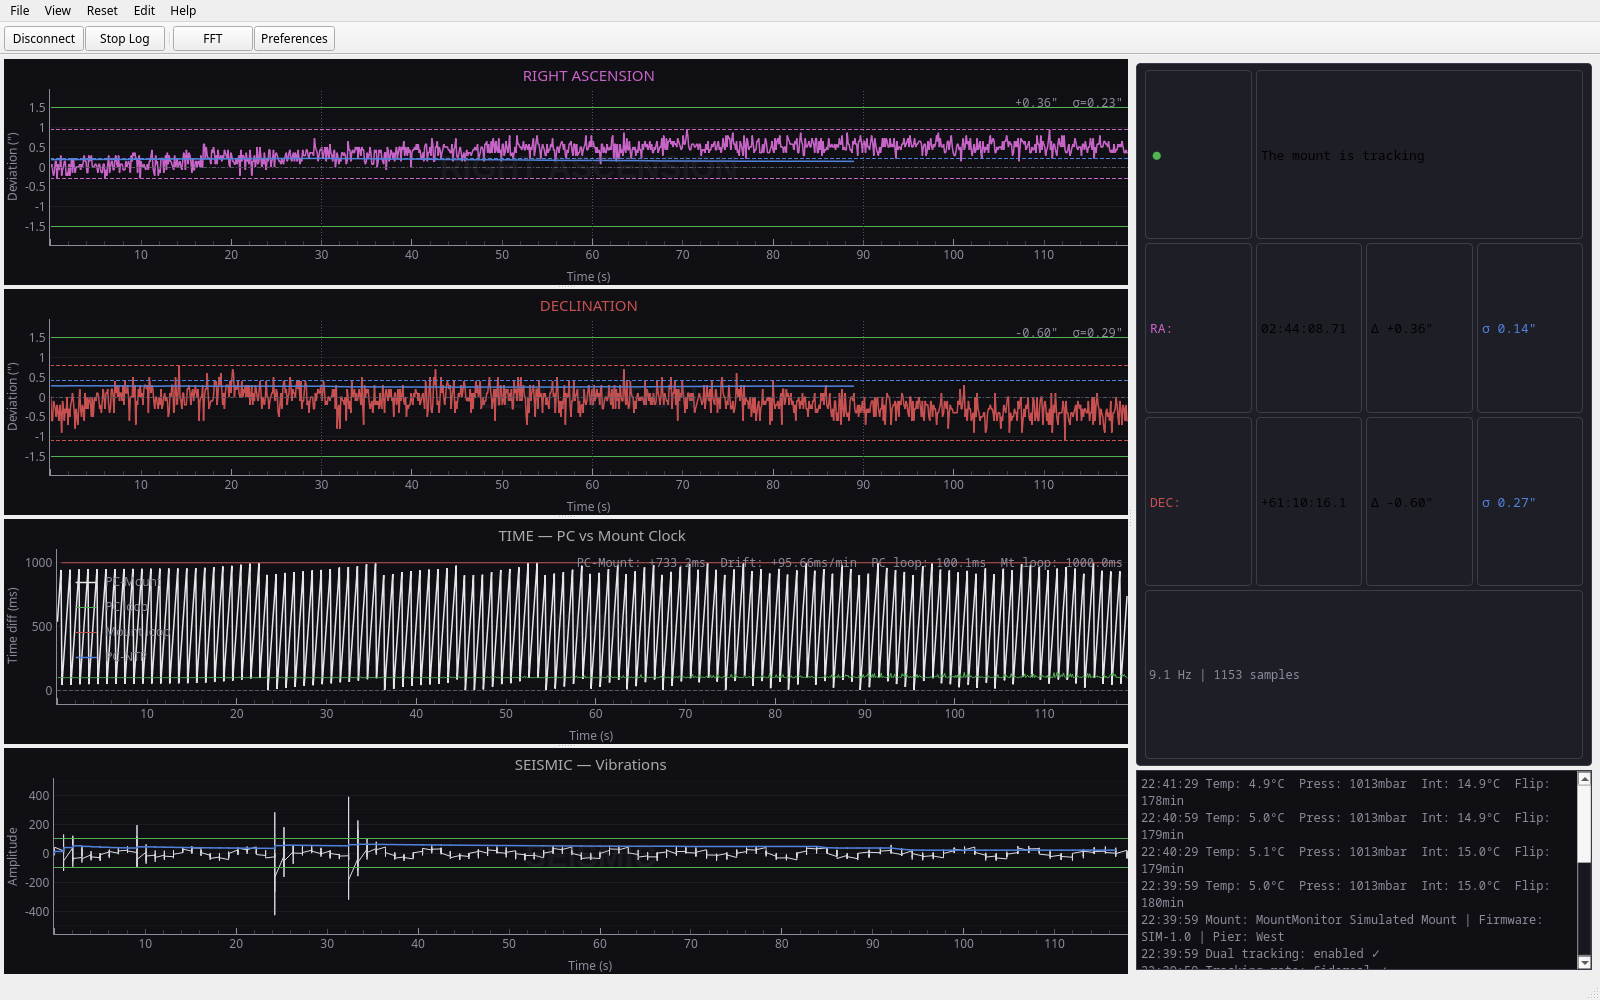
\includegraphics[width=\textwidth]{images/ecran_principal.png}
\caption{L'écran principal en fonctionnement. À gauche, les quatre graphes
empilés ; à droite, le bandeau d'état et le journal des messages.}
\end{figure}

\section{L'organisation}

L'écran se lit en deux colonnes.

\textbf{À gauche, les graphes}, toujours dans le même ordre, du haut vers le
bas :
\begin{enumerate}[nosep]
  \item \textsc{Right Ascension} --- l'ascension droite, en \pastille{accentmagenta}magenta ;
  \item \textsc{Declination} --- la déclinaison, en \pastille{accentred}rouge ;
  \item \textsc{Time} --- la comparaison des horloges ;
  \item \textsc{Seismic} --- les vibrations, si un sismomètre est branché.
\end{enumerate}

\textbf{À droite, l'état instantané} : un voyant, les coordonnées, les écarts,
et en dessous le journal qui défile.

\begin{tip}
L'ordre n'est pas décoratif. Les deux graphes du haut sont ceux qui décident
de la qualité de vos images. Celui du temps sert à savoir si les deux
premiers disent vrai. Celui du bas sert à savoir d'où vient le problème quand
il y en a un.
\end{tip}

\section{Le bandeau d'état}

\begin{figure}[H]
\centering
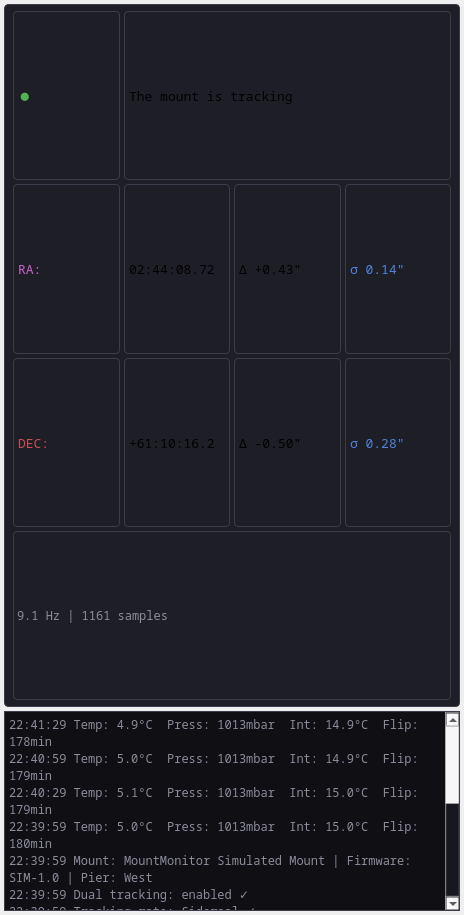
\includegraphics[width=0.42\textwidth]{images/bandeau_etat.png}
\caption{Le bandeau d'état : voyant, coordonnées brutes, écart instantané,
écart-type, cadence, puis le journal.}
\end{figure}

Ligne par ligne :

\begin{description}[leftmargin=2.2cm, style=nextline]
\item[Le voyant] Vert : la monture suit. Orange : elle pointe (elle se
déplace vers une cible). Gris : elle est parquée, ou à l'arrêt. Rouge :
erreur de communication.

\item[\texttt{RA: 02:44:08.72}] La position brute renvoyée par la monture,
telle quelle, en heures : minutes : secondes. C'est la réponse à la commande
\texttt{:GR\#}, sans retouche.

\item[\texttt{$\Delta$ +0.43\arcsec}] L'écart à la référence, en secondes
d'arc. Ce nombre devient rouge dès qu'il dépasse la tolérance que vous avez
fixée.

\item[\texttt{$\sigma$ 0.14\arcsec}] L'écart-type glissant : la dispersion des
dernières minutes. C'est le chiffre qui compte vraiment --- voir le
chapitre~\ref{ch:ad}.

\item[\texttt{9.1 Hz | 1161 samples}] La cadence réellement obtenue, et le
nombre d'échantillons depuis le début de la session.
\end{description}

\begin{warning}
\texttt{1161 samples} compte les échantillons \emph{depuis le début}, pas ceux
qui sont dans le graphe. Si la monture a pointé et que la remise à zéro
automatique est active, les graphes repartent à vide alors que ce compteur,
lui, continue. Une capture prise juste après un pointage montre donc une
seconde de données sous un compteur à plusieurs centaines --- ce n'est pas
une panne.
\end{warning}

\section{Le journal}

Sous le bandeau défile tout ce que le logiciel a remarqué : la connexion, les
contrôles de réglages de la monture, les dépassements de tolérance, les
relevés d'environnement, le temps restant avant le retournement au méridien.
Le plus récent est en haut.

\begin{tip}
C'est la première chose à relire le lendemain matin. Les dépassements de
tolérance y sont horodatés : vous savez à quelle heure ça s'est mal passé, et
vous n'avez plus qu'à regarder quelle image de votre série correspond.
\end{tip}

% ═══════════════════════════════════════════════════════════════════
\chapter{Le graphe d'ascension droite}
\label{ch:ad}

C'est le graphe le plus important, et celui qui contient le plus de choses.
On va le démonter élément par élément.

\begin{figure}[H]
\centering
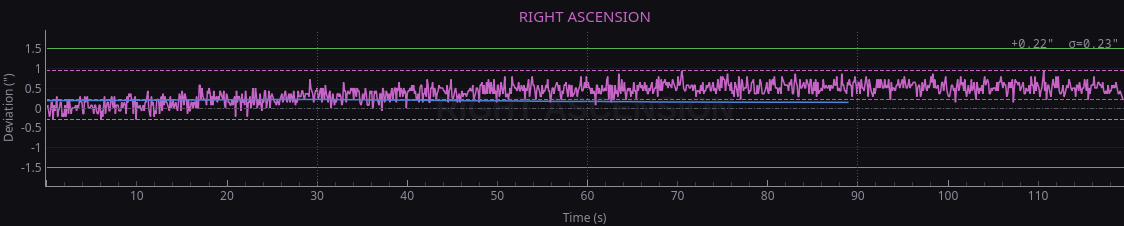
\includegraphics[width=\textwidth]{images/graphe_ad.png}
\caption{Le graphe d'ascension droite. La courbe magenta est la donnée ; tout
le reste sert à la juger.}
\end{figure}

\section{L'axe vertical : des secondes d'arc}

\begin{simple}
La hauteur, c'est l'erreur de suivi, en secondes d'arc. Zéro au milieu : la
monture est là où elle devrait être. Plus la courbe s'éloigne du centre, plus
l'étoile a bougé sur le capteur.
\end{simple}

\begin{prepa}
Une seconde d'arc vaut $1/3600$ de degré. Ce qu'elle représente sur vos
images dépend entièrement de l'instrument :

\begin{center}
\begin{tabular}{lrrr}
\toprule
\textbf{Instrument} & \textbf{Focale} & \textbf{Échantillonnage} & \textbf{1\,\arcsec vaut} \\
\midrule
RC10 CFF f/8 & \SI{2000}{\milli\meter} & 0,39\,\arcsec/pixel & 2,6 pixels \\
FSQ-106 f/5 & \SI{530}{\milli\meter} & 1,46\,\arcsec/pixel & 0,7 pixel \\
FC-76DCU f/7,5 & \SI{570}{\milli\meter} & 1,36\,\arcsec/pixel & 0,7 pixel \\
\bottomrule
\end{tabular}
\end{center}

\noindent (capteurs à photosites de \SI{3,76}{\micro\meter} ; valeurs
produites par \texttt{echantillonnage.py}).
\end{prepa}

\begin{avance}
L'ascension droite est un angle \emph{sur l'équateur céleste}. Mais l'étoile
que vous photographiez n'est pas forcément sur l'équateur : à la déclinaison
$\delta$, un déplacement de $1\,\arcsec$ en ascension droite ne déplace
l'image que de $1'' \times \cos\delta$. À $\delta = 60^\circ$, le
facteur vaut $0,5$ : l'erreur affichée est deux fois plus grande que celle
qui atteint vos pixels. Le logiciel affiche la valeur \emph{angulaire brute}
en secondes d'arc ; c'est à vous de faire le pas vers le capteur --- sauf si
vous activez l'option décrite au \S\ref{sec:ha}, qui fait la conversion.
\end{avance}

\section{Les lignes, une par une}

\subsection{\pastille{accentmagenta}La courbe magenta : la donnée}

L'écart mesuré à chaque échantillon. Elle est bruitée, c'est normal : elle
contient le bruit de la mesure elle-même (retard réseau, arrondi de la
monture) autant que le mouvement réel de la monture.

\subsection{\pastille{accentblue}La courbe bleue ondulante : l'écart-type glissant}

\begin{simple}
Elle ne monte pas quand l'erreur est grande : elle monte quand l'erreur est
\emph{agitée}. Une monture décalée de deux secondes d'arc mais parfaitement
stable donne une courbe bleue plate et basse --- et des étoiles rondes.
\end{simple}

\begin{prepa}
C'est l'écart-type calculé sur une fenêtre glissante de 60, 120, 300 ou
\SI{900}{\second}, au choix. Ces quatre durées ne sont pas arbitraires : ce
sont celles qu'utilise le service technique de 10Micron pour analyser les
journaux de ses montures. Choisir la même permet de comparer ce que vous
voyez à ce qu'ils voient.
\end{prepa}

\begin{avance}
L'écart-type glissant est un filtre passe-haut déguisé : il ignore tout ce
qui est plus lent que sa fenêtre. Une dérive de 5\,\arcsec/h
laisse la courbe bleue parfaitement plate sur une fenêtre de
\SI{60}{\second}, parce que sur une minute cette dérive ne représente que
0,08\,\arcsec --- noyés dans le bruit. C'est voulu : la dérive se lit
sur la courbe magenta, l'agitation sur la bleue. Deux défauts différents,
deux instruments de mesure différents.

\medskip
Conséquence pratique : \textbf{la courbe bleue est en retard}. Calculée sur
les $N$ dernières secondes, elle atteint son maximum environ $N/2$ après
l'événement qui l'a causé. Le réglage \emph{Corriger les graphes de la
longueur de fenêtre} décale la courbe de $N/2$ pour recaler le pic sur sa
cause. Activez-le : sans lui, vous cherchez la perturbation au mauvais
endroit.
\end{avance}

\subsection{\pastille{accentgreen}Les traits verts horizontaux : les tolérances}

Vos seuils, fixés dans les préférences, de part et d'autre de la référence.
Quand la donnée ou l'écart-type les dépasse, un message part dans le journal
et le chiffre du bandeau passe au rouge.

\begin{tip}
Quelle tolérance choisir ? Celle en dessous de laquelle le défaut ne se voit
pas sur l'image. Au RC10, la turbulence de votre site étale déjà chaque
étoile sur 6 à 9 pixels (seeing de 2,5 à 3,5\arcsecond). Une erreur de suivi
de 1\,\arcsec y ajoute 2,6 pixels : elle commence à compter. Une
erreur de 0,3\,\arcsec disparaît dans la turbulence. À la FSQ, avec
1,46\,\arcsec par pixel, il faut près de 1,5\,\arcsec d'erreur
pour déplacer l'étoile d'un seul pixel.
\end{tip}

\subsection{Les pointillés horizontaux : les extrêmes}

Le minimum et le maximum rencontrés depuis la dernière remise à zéro, avec
leur valeur annotée. Ils ne redescendent jamais tout seuls : un unique coup de
vent laisse sa trace toute la nuit. C'est le but --- mais cela veut dire qu'un
écart maximal de 4\,\arcsec ne signifie pas que le suivi était mauvais,
seulement qu'il a été mauvais \emph{une fois}.

\subsection{Les traits verticaux gris : les repères de temps}

Un toutes les 30 secondes, annoté avec l'heure de la monture. Ils servent à
relier un accident du graphe à une image précise de votre série.

\section{L'écart-type, le seul chiffre à retenir}
\label{sec:sigma}

\begin{formula}
\[
\sigma = \sqrt{\frac{1}{N}\sum_{i=1}^{N}\left(x_i - \bar{x}\right)^2}
\]
où les $x_i$ sont les $N$ écarts mesurés pendant la fenêtre glissante.
\end{formula}

\begin{simple}
Si vous ne deviez regarder qu'un nombre de tout l'écran, ce serait le
$\sigma$ du bandeau. Il résume en un chiffre l'agitation de la monture. En
dessous de la moitié de votre seeing, vous êtes tranquille.
\end{simple}

\begin{avance}
Pourquoi l'écart-type et pas l'écart maximal ? Parce que l'image intègre. Une
pose de cinq minutes additionne toutes les positions prises par l'étoile
pendant ces cinq minutes : le résultat est une tache dont la largeur est la
\emph{somme quadratique} de la tache de seeing et de l'agitation de suivi,
pas la somme des extrêmes.

\[
\text{FWHM}_{\text{image}} \simeq \sqrt{\text{FWHM}_{\text{seeing}}^2
+ \left(2{,}35\,\sigma_{\text{suivi}}\right)^2}
\]

Le facteur $2{,}35$ convertit un écart-type en largeur à mi-hauteur pour une
distribution normale. À un seeing de 3\,\arcsec et un
$\sigma$ de 0,5\,\arcsec, la dégradation est de
$\sqrt{3^2 + 1{,}18^2} = 3{,}22\arcsecond$, soit \SI{7}{\percent} : invisible.
Au même seeing avec $\sigma = 1,5\,\arcsec$, on passe à
$\SI{4,7}{\arcsecond}$, soit \SI{57}{\percent} de plus : là, ça se voit.
\end{avance}

% ═══════════════════════════════════════════════════════════════════
\chapter{Le graphe de déclinaison}

\begin{figure}[H]
\centering
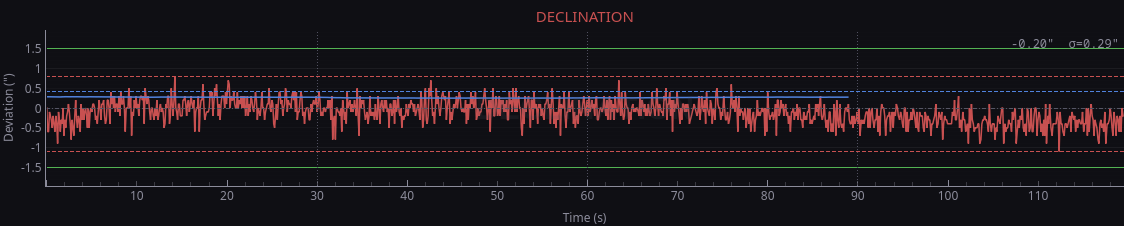
\includegraphics[width=\textwidth]{images/graphe_dec.png}
\caption{Le graphe de déclinaison. Mêmes éléments que celui d'ascension
droite ; la donnée est en rouge.}
\end{figure}

Tout ce qui a été dit du graphe d'ascension droite vaut ici, à une couleur
près. Ce qui change, c'est l'\emph{interprétation}.

\section{Pourquoi les deux axes ne fautent pas pareil}

\begin{simple}
En ascension droite, la monture tourne en permanence pour suivre le ciel :
tout ce qui cloche dans cette rotation se voit. En déclinaison, elle ne
devrait pas bouger du tout. Une erreur en déclinaison n'a donc pas les mêmes
causes qu'une erreur en ascension droite.
\end{simple}

\begin{prepa}
L'axe d'ascension droite tourne à la vitesse sidérale,
15,041\,\arcsec/s à l'équateur céleste. Il porte donc :
\begin{itemize}[nosep]
  \item l'\textbf{erreur périodique} de son entraînement (une ondulation
  régulière dont la période est celle de la vis sans fin) ;
  \item les défauts de vitesse ;
  \item la part d'erreur d'alignement polaire qui se projette sur cet axe.
\end{itemize}
L'axe de déclinaison, lui, est immobile en suivi. Une dérive lente et
régulière en déclinaison ne peut venir que de trois choses : l'alignement
polaire, la réfraction atmosphérique, ou une flexion mécanique.
\end{prepa}

\begin{tip}
La règle de dépannage que MountMonitor applique lui-même dans son rapport de
nuit :
\begin{itemize}[nosep]
  \item dérive en \textbf{ascension droite} $\rightarrow$ regardez
  l'\textbf{azimut} de l'alignement polaire ;
  \item dérive en \textbf{déclinaison} $\rightarrow$ regardez
  l'\textbf{altitude} (la hauteur) de l'alignement polaire.
\end{itemize}
Au-delà de 5\,\arcsec/h, il vous le dit en toutes lettres.
\end{tip}

\begin{avance}
Avec un modèle de pointage à jour --- et votre GM1000 en a un --- la monture
corrige elle-même l'essentiel de l'erreur d'alignement polaire et de la
réfraction. Ce que vous observez alors en déclinaison n'est plus l'erreur
d'alignement, mais l'\emph{erreur résiduelle du modèle}, c'est-à-dire ce que
le modèle n'a pas su prédire : flexion différentielle, jeu mécanique,
variation de réfraction depuis la construction du modèle. Une dérive en
déclinaison qui apparaît au fil de la nuit alors que le modèle est bon
signale en général un changement de température ou une charge qui a bougé, pas
un alignement à refaire.
\end{avance}

\section{L'option « tolérance en secondes de temps »}
\label{sec:ha}

C'est le réglage le plus déroutant de tout le logiciel. Voici ce qu'il fait.

\begin{prepa}
L'ascension droite se mesure naturellement en \emph{temps} : \SI{24}{\hour}
font un tour complet. Une seconde de temps vaut donc 15\,\arcsec
d'angle --- à l'équateur céleste seulement. Ailleurs, le cercle parcouru est
plus petit d'un facteur $\cos\delta$.

\begin{formula}
\[
\text{écart en secondes de temps} =
\frac{\text{écart en secondes d'arc}}{15 \times \cos\delta}
\]
\end{formula}

Quand l'option est active, le bandeau affiche
\texttt{$\Delta$ +0.029s} au lieu de \texttt{$\Delta$ +0.43\arcsec}, et les
traits verts de tolérance sont tracés à la même échelle que ce que rapporte
la monture.
\end{prepa}

\begin{warning}
Les deux lectures ne sont pas interchangeables. En secondes de temps, vous
comparez l'erreur à ce que la monture \emph{croit} faire. En secondes d'arc,
vous la comparez à ce qui arrive \emph{à votre capteur}. Pour décider si une
nuit est bonne, c'est la seconde d'arc qui compte. L'option existe pour
dialoguer avec les outils de 10Micron, qui raisonnent en temps.
\end{warning}

% ═══════════════════════════════════════════════════════════════════
\chapter{Vitesse et déplacement axiaux}

Ce graphe n'existe que sur les montures 10Micron, et il ne s'affiche que si
vous l'activez. C'est le plus riche du logiciel, et le moins connu.

\begin{figure}[H]
\centering
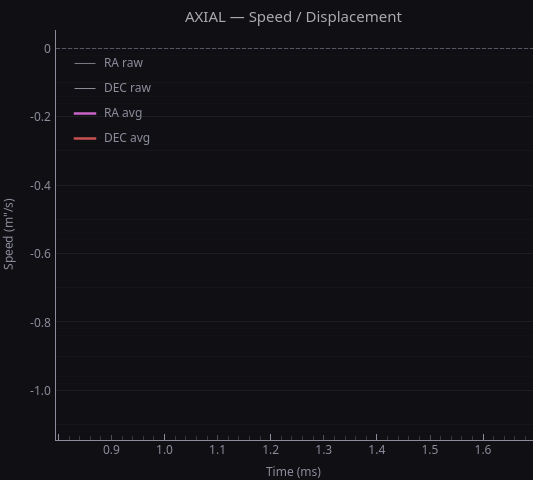
\includegraphics[width=0.62\textwidth]{images/graphe_axial.png}
\caption{Le graphe axial. Trois tracés de la même grandeur, lissés
différemment.}
\end{figure}

\section{D'où viennent ces données}

\begin{simple}
Les graphes précédents disent où la monture \emph{croit pointer}. Celui-ci
dit à quelle vitesse ses axes \emph{tournent réellement}. Ce n'est pas la
même question, et la réponse est souvent plus parlante.
\end{simple}

\begin{prepa}
Depuis la version 3.20 de son firmware, une 10Micron répond à deux commandes
supplémentaires : \texttt{:GaXa\#} et \texttt{:GaXb\#}, qui rendent
l'orientation brute de l'axe d'ascension droite et de celui de déclinaison.
En dérivant cette orientation par rapport au temps, on obtient une vitesse ;
en l'intégrant, un déplacement.

Sans erreur d'alignement polaire et sans réfraction, ces vitesses devraient
valoir :
\begin{itemize}[nosep]
  \item 15,02\,\arcsec/s pour l'ascension droite ;
  \item 0\,\arcsec/s pour la déclinaison.
\end{itemize}
Tout écart à ces deux valeurs est une correction que la monture applique --- ou
un défaut qu'elle subit.
\end{prepa}

\section{Les trois tracés, et pourquoi il y en a trois}

\begin{description}[leftmargin=0.5cm, style=nextline]
\item[Le tracé gris, fin : la vitesse brute]
Calculée entre deux échantillons consécutifs seulement. C'est la mesure la
plus honnête et la plus bruyante : le moindre retard réseau entre la question
et la réponse s'y traduit par une fausse variation de vitesse.

\item[Le tracé noir épais : la moyenne sur six échantillons]
Le même signal, moyenné. Le bruit de mesure s'efface, le mouvement réel
reste.

\item[Le tracé noir très épais : la régression linéaire]
Une droite ajustée sur toute la longueur de la fenêtre glissante. Très
lisse, très lisible --- mais elle efface les petites variations et elle
\emph{retarde} le graphe de la longueur de la fenêtre.
\end{description}

\begin{avance}
Ces trois tracés forment un compromis biais--variance explicite, offert à
l'\oe{}il de l'utilisateur au lieu d'être tranché à sa place. La dérivation
numérique amplifie le bruit : si l'incertitude sur une position est
$\sigma_x$ et l'intervalle d'échantillonnage $\Delta t$, l'incertitude sur la
vitesse à deux points vaut $\sigma_v = \sigma_x\sqrt{2}/\Delta t$. À
\SI{9,1}{\hertz} et $\sigma_x = 0{,}1\,\arcsec$, cela fait déjà
1,3\,\arcsec/s de bruit --- du même ordre que les défauts
qu'on cherche. Moyenner sur $n$ points divise ce bruit par $\sqrt{n}$, au prix
d'un retard de $n/2$ échantillons. La régression sur toute la fenêtre pousse
le raisonnement à son terme.
\end{avance}

\section{Le déplacement, et la valeur « SPH »}

En choisissant l'affichage en déplacement plutôt qu'en vitesse, le troisième
tracé est remplacé par l'intégrale de la vitesse : de combien l'axe s'est
effectivement déplacé.

\begin{prepa}
Le graphe est alors annoté de deux valeurs :
\begin{itemize}[nosep]
  \item le déplacement en secondes d'arc, \texttt{[x.xx\arcsec]} ;
  \item le déplacement \emph{sphérique}, \texttt{[x.xx\arcsec SPH]},
  c'est-à-dire le précédent multiplié par $\cos\delta$.
\end{itemize}
\end{prepa}

\begin{tip}
C'est la valeur SPH, et elle seule, qu'il faut comparer à la taille d'un
pixel. Au RC10, un pixel vaut 0,39\,\arcsec : un déplacement
sphérique de 0,4\,\arcsec\,SPH a bougé l'étoile d'un pixel, quelle que
soit la déclinaison de la cible. C'est aussi la grandeur qui se compare
directement à ce qu'affiche PHD2.
\end{tip}

\begin{warning}
Les deux premières minutes de ce graphe ne valent rien. Le logiciel attend
cent échantillons avant de tenter la moindre régression, et l'aide officielle
du MountMonitor d'origine prévient qu'il faut au moins \emph{deux fois} la
longueur de la fenêtre glissante avant que les valeurs soient fiables. Avec
une fenêtre de \SI{300}{\second}, cela fait dix minutes : ne concluez rien
avant.
\end{warning}

% ═══════════════════════════════════════════════════════════════════
\chapter{Le graphe du temps}

C'est le graphe que personne ne regarde, et c'est celui qui sauve les nuits
inexplicables.

\begin{figure}[H]
\centering
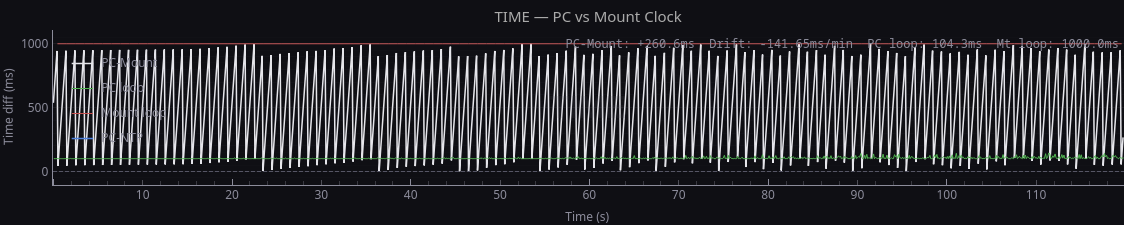
\includegraphics[width=\textwidth]{images/graphe_temps.png}
\caption{Le graphe du temps. Quatre courbes, quatre horloges comparées.}
\end{figure}

\section{Pourquoi comparer des horloges}

\begin{simple}
La monture sait où pointer \emph{si} elle sait quelle heure il est. Une
horloge qui dérive, c'est un ciel qui n'est pas là où la monture le croit. Ce
graphe vérifie que l'ordinateur et la monture sont d'accord sur l'heure.
\end{simple}

\begin{prepa}
Le ciel tourne à 15,041\,\arcsec/s. Une erreur d'horloge
d'une seule seconde déplace donc la cible de 15\,\arcsec en ascension
droite --- soit, au RC10, \num{39} pixels. Une erreur de
\SI{100}{\milli\second} en déplace déjà \num{4}. C'est pour cela que le
logiciel mesure les horloges à la milliseconde.
\end{prepa}

\section{Les quatre courbes}

\begin{description}[leftmargin=0.5cm, style=nextline]
\item[\pastille{white}La courbe blanche : PC $-$ monture]
La différence entre l'heure de l'ordinateur et celle de la monture. C'est la
courbe principale. Une ligne horizontale, même décalée de zéro, est bonne
nouvelle : les deux horloges avancent du même pas.

\item[\pastille{accentgreen}La courbe verte : la boucle vue par le PC]
Le temps qu'a pris un tour complet d'interrogation, mesuré par l'horloge de
l'ordinateur.

\item[\pastille{accentred}La courbe rouge : la boucle vue par la monture]
Le même tour, mesuré par l'horloge de la monture.

\item[\pastille{accentblue}La courbe bleue : PC $-$ serveur de temps]
L'écart entre l'ordinateur et un serveur de temps du réseau, quand il y en a
un de configuré.
\end{description}

\begin{tip}
Quand tout va bien, \textbf{la rouge est cachée sous la verte} : les deux
horloges mesurent la même durée pour le même tour. On ne voit du rouge qu'aux
pics.
\end{tip}

\section{Lire un saut d'horloge --- et savoir qui a sauté}

C'est l'usage le plus fin de ce graphe, et il mérite d'être compris une fois
pour toutes.

\begin{prepa}
Quand la courbe blanche fait un saut brutal, deux coupables sont possibles :
l'horloge du PC ou celle de la monture. On les distingue en regardant
\emph{quel bord} du saut porte une couleur :
\begin{itemize}[nosep]
  \item une amorce \textbf{verte} le long du front du saut $\rightarrow$
  c'est l'horloge du \textbf{PC} qui a sauté (une synchronisation réseau, par
  exemple) ;
  \item une amorce \textbf{rouge} $\rightarrow$ c'est l'horloge de la
  \textbf{monture}.
\end{itemize}
\end{prepa}

\begin{avance}
Le raisonnement est le suivant. La courbe blanche est une \emph{différence} :
elle ne dit pas lequel des deux termes a bougé. Les courbes verte et rouge
mesurent la \emph{même durée physique} --- un tour d'interrogation --- avec
deux horloges différentes. Si le PC saute d'une seconde pendant un tour, le
tour dure une seconde de plus selon le PC seulement : la verte fait un pic,
la rouge non. Si c'est la monture, c'est l'inverse. La différence commune
s'annule, le désaccord reste : c'est une mesure différentielle, et c'est ce
qui lui donne son pouvoir de discrimination.

\medskip
Conséquence concrète documentée par l'auteur du logiciel d'origine : une
synchronisation d'horloge de la monture \emph{pendant le suivi} provoque un
saut de 1,18\,\arcsec en ascension droite --- un filé d'étoile sur
l'image en cours. Ne laissez jamais un utilitaire synchroniser l'heure de la
monture pendant une acquisition.
\end{avance}

\begin{warning}
Les courbes verte et rouge sont tracées avec un décalage vertical volontaire,
calculé par une moyenne glissante, pour qu'elles tiennent à l'écran avec la
blanche. Leur position absolue ne veut donc rien dire ; seules comptent leurs
variations. La blanche, elle, n'a pas de décalage : le trait gris horizontal
au centre est le vrai zéro.
\end{warning}

% ═══════════════════════════════════════════════════════════════════
\chapter{Le graphe sismique}

\begin{figure}[H]
\centering
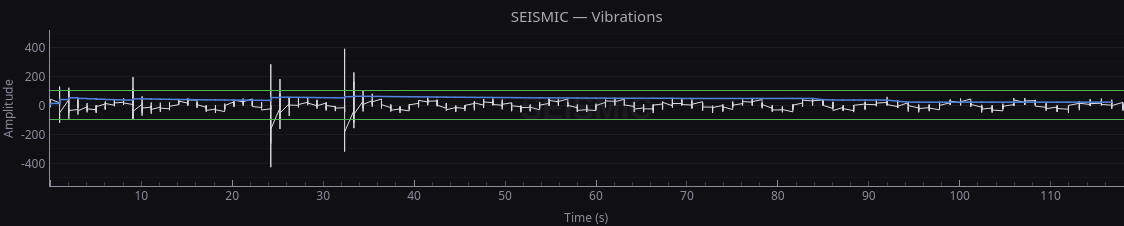
\includegraphics[width=\textwidth]{images/graphe_sismique.png}
\caption{Le graphe sismique. Il ne mesure pas la monture, mais le sol sous
ses pieds.}
\end{figure}

\begin{simple}
Cette courbe ne vient pas de la monture : elle vient d'un petit capteur de
vibrations branché à l'ordinateur. Elle répond à une question précise :
« est-ce que ce que je vois dans les deux graphes du haut vient de la monture,
ou de quelque chose qui a secoué le sol ? »
\end{simple}

\begin{prepa}
L'échelle verticale est \emph{manuelle} --- vous la fixez dans les
préférences --- contrairement aux graphes d'ascension droite et de
déclinaison, dont l'échelle s'ajuste seule. C'est délibéré : les unités d'un
sismomètre amateur sont arbitraires, seules comptent les variations relatives
et la répétition des événements.

La courbe bleue est, comme ailleurs, l'écart-type glissant ; les traits verts
sont la tolérance, exprimée ici en pourcentage de l'amplitude.
\end{prepa}

\begin{avance}
Le sismomètre est échantillonné bien plus vite que la monture --- typiquement
\SI{20}{\hertz} contre \SI{2}{\hertz} à \SI{10}{\hertz}. Ce n'est pas un
luxe : par Nyquist--Shannon, cela repousse la limite de détection à
\SI{10}{\hertz}, où vivent les résonances mécaniques d'un trépied, d'un pilier
ou d'un plancher. Les données de monture, elles, ne voient rien au-dessus de
quelques hertz.

\medskip
C'est tout l'intérêt de la corrélation : une perturbation visible dans le
spectre sismique \emph{et} dans le spectre d'ascension droite à la même
fréquence a une cause commune extérieure. Une perturbation visible dans
l'ascension droite seule est mécanique, dans la monture.
\end{avance}

\begin{tip}
Le cas d'école : une vibration régulière vers \SI{1}{\hertz} qui apparaît sur
le sismique et sur l'ascension droite quand quelqu'un marche à proximité, ou
quand le vent force. Sans le sismomètre, on accuse la monture ; avec, on
déplace le pied ou on attend que le vent tombe.
\end{tip}

% ═══════════════════════════════════════════════════════════════════
\chapter{La fenêtre FFT}

\begin{figure}[H]
\centering
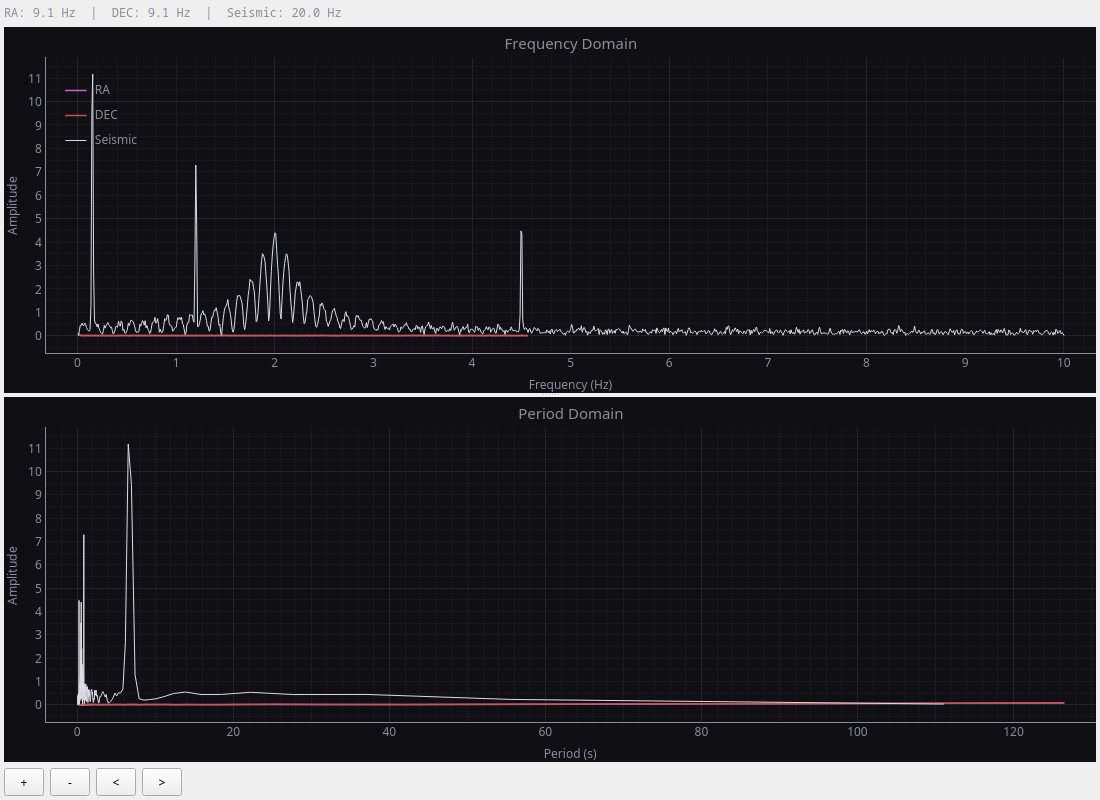
\includegraphics[width=\textwidth]{images/fenetre_fft.png}
\caption{La fenêtre d'analyse fréquentielle. En haut le domaine des
fréquences, en bas celui des périodes.}
\end{figure}

\section{Ce que fait une transformée de Fourier}

\begin{simple}
Les graphes principaux montrent l'erreur \emph{au fil du temps}. Celui-ci
montre de quoi cette erreur est \emph{faite} : une bosse à
\SI{0,002}{\hertz} veut dire qu'il existe dans votre suivi une ondulation qui
revient toutes les huit minutes. Il ne reste plus qu'à trouver ce qui, dans
la monture, tourne en huit minutes.
\end{simple}

\begin{prepa}
La transformée de Fourier décompose un signal en somme de sinusoïdes. La
hauteur d'un pic donne l'amplitude de la composante, sa position en donne la
fréquence. La fenêtre affiche les deux lectures du même résultat :
\begin{itemize}[nosep]
  \item en \textbf{fréquence} (Hz) en haut : pratique pour les vibrations ;
  \item en \textbf{période} (secondes) en bas : pratique pour l'erreur
  périodique, dont on connaît la durée de cycle.
\end{itemize}
En haut à droite, les cadences réelles de chaque source sont rappelées, dans
la couleur de leur courbe.
\end{prepa}

\begin{avance}
Trois mises en garde que la lecture naïve d'un spectre ignore.

\medskip
\textbf{La limite de Nyquist.} Le spectre s'arrête à la moitié de la cadence
d'échantillonnage. À \SI{9,1}{\hertz}, rien au-delà de \SI{4,55}{\hertz}.
Pire : une vibration à \SI{6}{\hertz} ne disparaît pas, elle se replie et
apparaît à \SI{3,5}{\hertz}, parfaitement crédible et complètement fausse.

\medskip
\textbf{La résolution fréquentielle.} Elle vaut $1/T$ où $T$ est la durée
observée. Pour distinguer deux raies distantes de \SI{0,001}{\hertz}, il faut
\SI{1000}{\second} de données, soit un quart d'heure. Un spectre calculé sur
deux minutes ne peut rien dire des périodes de plus de deux minutes.

\medskip
\textbf{La fenêtre d'apodisation.} Le logiciel applique une fenêtre de Hann
avant la transformation, et retire la moyenne. Sans cela, la troncature du
signal étale chaque raie sur tout le spectre --- des pics fantômes partout.
C'est indispensable, et cela élargit légèrement les raies réelles : une raie
isolée dans le spectre correspond à une oscillation un peu plus pure qu'elle
n'en a l'air.
\end{avance}

\section{Lecture de la figure ci-dessus}

Prenons la capture de ce chapitre, et lisons-la comme on lirait la vôtre.

\begin{enumerate}
\item \textbf{L'en-tête} annonce \texttt{RA: 9.9 Hz | DEC: 9.9 Hz |
Seismic: 20.0 Hz}. Les données de monture sont donc échantillonnées à
\SI{9,9}{\hertz} : le spectre du haut n'a de sens pour elles que jusqu'à
\SI{4,95}{\hertz}. Le sismomètre, à \SI{20}{\hertz}, porte jusqu'à
\SI{10}{\hertz} --- et c'est bien jusqu'à \num{10} que va l'axe.

\item \textbf{Les courbes magenta et rouge sont plates.} L'ascension droite
et la déclinaison ne contiennent aucune composante périodique marquée : le
suivi est propre.

\item \textbf{La courbe blanche, elle, a du relief.} Une raie très fine vers
\SI{0,15}{\hertz}, une autre vers \SI{1,2}{\hertz}, une bosse large centrée
sur \SI{2}{\hertz}, une raie nette vers \SI{4,5}{\hertz}.

\item \textbf{Raie fine contre bosse large.} Une raie fine est une source
mécanique régulière : quelque chose qui tourne ou qui oscille à sa fréquence
propre. Une bosse large est un phénomène sans période franche --- du vent, du
passage, de la turbulence.

\item \textbf{Le domaine des périodes, en bas}, dit la même chose dans
l'autre langue : le pic à \SI{6,5}{\second} de période est le même objet que
la raie à \SI{0,15}{\hertz} du haut. Pour une erreur périodique de vis sans
fin, dont le catalogue donne la durée de cycle en secondes, c'est ce
graphe-là qu'on lit.
\end{enumerate}

\begin{warning}
Ici, rien de tout cela n'atteint la monture : les courbes magenta et rouge
restent plates malgré l'agitation sismique. C'est exactement le genre de
conclusion qu'on ne peut pas tirer sans les deux mesures côte à côte --- et
c'est la raison d'être de cette fenêtre.
\end{warning}

\begin{tip}
Sur une GM1000, l'erreur périodique résiduelle est faible, et le modèle de
pointage en absorbe une bonne part. Ce que vous chercherez plutôt dans ce
spectre, ce sont des raies \emph{basses} --- quelques minutes de période ---
signant une flexion ou un déséquilibre, et des raies \emph{hautes} communes
au sismique, signant l'environnement.
\end{tip}

% ═══════════════════════════════════════════════════════════════════
\chapter{Le rapport de nuit}

Quand la monture se parque, MountMonitor relit tout ce qu'il a enregistré et
en tire un rapport. C'est le seul écran que vous lirez le lendemain, au
calme.

\section{Ce qu'il contient}

Treize sections, dont les plus utiles sont :

\begin{center}
\begin{tabularx}{\textwidth}{lX}
\toprule
\textbf{Section} & \textbf{Ce qu'elle vous apprend} \\
\midrule
Note de qualité & Un verdict global sur la nuit, pour trier vite. \\
Statistiques AD / DÉC & Moyenne, médiane, écart-type, percentiles, extrêmes. \\
Analyse des tolérances & Le pourcentage d'échantillons au-delà de 0,5\,\arcsec,
1\,\arcsec, 2\,\arcsec\ldots{} C'est la vraie mesure de la nuit. \\
Dérive & La pente, en secondes d'arc par heure, et l'axe d'alignement à
corriger. \\
FFT / erreur périodique & Les périodes dominantes trouvées. \\
Statut de suivi & Le temps passé réellement en suivi, et le reste. \\
Environnement & Température, pression, points de rosée relevés. \\
Recommandations & Ce que le logiciel conclut, en clair. \\
\bottomrule
\end{tabularx}
\end{center}

\begin{tip}
La ligne à lire en premier est celle des \textbf{percentiles}. « 95\% des
échantillons sous 0,6\,\arcsec » vous dit tout ; le maximum, lui, ne
décrit qu'un instant, souvent un coup de vent.
\end{tip}

\begin{warning}
Le rapport ne juge que la \emph{stabilité}, pas la \emph{justesse}. Une
monture parfaitement stable mais décalée de dix secondes d'arc de la cible
obtient une excellente note : c'est le choix de la médiane comme référence
qui le veut (\S\ref{ch:ad}). Pour vérifier la justesse, il faut passer la
référence sur les coordonnées de cible.
\end{warning}

\section{Analyse d'un journal déjà enregistré}

Le menu \emph{Fichier} permet de rouvrir n'importe quel \texttt{.dat} d'une
nuit passée : les graphes se remplissent comme si la nuit recommençait, la
FFT se recalcule, et le rapport s'ouvre. C'est l'outil à utiliser quand une
série d'images s'est mal passée et que vous voulez savoir pourquoi.

\begin{prepa}
Les fichiers d'une session portent tous le même préfixe horodaté et
diffèrent par l'extension :
\begin{itemize}[nosep]
  \item \texttt{.log} --- les événements, en clair ;
  \item \texttt{.dat} --- les données de monture, 27 colonnes séparées par des
  tabulations ;
  \item \texttt{.dti} --- les mesures de temps ;
  \item \texttt{.sei} --- le sismomètre ;
  \item \texttt{.fft} --- les spectres successifs ;
  \item \texttt{.env} --- l'environnement et les diagnostics.
\end{itemize}
Tous sont du texte : un tableur les ouvre directement.
\end{prepa}

% ═══════════════════════════════════════════════════════════════════
\chapter{Les réglages qui changent ce que vous voyez}

Quatre réglages modifient l'affichage au point qu'on peut croire à une panne.
Les voici.

\section{Le zoom vertical, quatre modes}

\begin{center}
\begin{tabularx}{\textwidth}{lX}
\toprule
\textbf{Mode} & \textbf{Effet} \\
\midrule
Données (centré médiane) & L'échelle suit les données. Les traits de
tolérance peuvent sortir de l'écran. \\
Tolérance & L'échelle suit les tolérances. Les données peuvent sortir de
l'écran. \\
Maximum & Les deux tiennent à l'écran. Un pic isolé écrase alors tout le
reste. \\
Lignes min/max & L'échelle suit les extrêmes rencontrés. \\
\bottomrule
\end{tabularx}
\end{center}

\begin{warning}
En mode « Données », une courbe qui remplit tout l'écran \emph{ne veut rien
dire} tant qu'on n'a pas regardé la graduation : l'échelle s'est ajustée. Une
nuit excellente et une nuit catastrophique se ressemblent, à la graduation
près. C'est la cause numéro un des frayeurs inutiles.
\end{warning}

\section{Le zoom horizontal}

Il fixe combien de données tiennent en largeur : au zoom 1, un point de
donnée par pixel d'écran ; au zoom 5, cinq pixels par point, donc cinq fois
moins d'histoire visible, mais en détail.

\section{La longueur de la fenêtre glissante}

60, 120, 300 ou \SI{900}{\second}. Elle commande l'écart-type, la vitesse
axiale et le déplacement axial. Plus elle est longue, plus les courbes sont
lisses --- et plus elles sont en retard.

\section{La remise à zéro automatique au pointage}

Par défaut, les tampons et les graphes se vident quand la monture pointe une
nouvelle cible : chaque cible repart d'une page blanche. C'est ce qui
explique qu'un graphe puisse afficher une seconde de données alors que le
compteur d'échantillons en annonce plusieurs centaines.

% ═══════════════════════════════════════════════════════════════════
\chapter{Trois lectures, sur votre matériel}

Assez de théorie. Voici trois situations concrètes, avec le raisonnement
complet.

\section{« Mes étoiles sont allongées sur les poses du RC10 »}

\begin{enumerate}
\item \textbf{Regardez le $\sigma$, pas la courbe.} Au RC10
(0,39\,\arcsec par pixel) et sous un seeing de
2,5 à 3,5\,\arcsec, la turbulence étale déjà chaque étoile sur
6 à 9 pixels. Un $\sigma$ de 0,3\,\arcsec n'y ajoute rien de visible ;
un $\sigma$ de 1,5\,\arcsec élargit la tache de plus de la moitié.

\item \textbf{Comparez l'ascension droite et la déclinaison.} Un allongement
dans une seule direction se retrouve sur un seul des deux graphes. Si les
deux $\sigma$ sont comparables, la cause est extérieure : vent, sol,
turbulence.

\item \textbf{Ouvrez la FFT.} Une raie nette à une période de quelques minutes
signe un défaut mécanique ; un plateau large signe de la turbulence, qui n'a
pas de période.

\item \textbf{Regardez le graphe du temps.} Un saut d'horloge pendant la pose
donne un filé net, et lui seul.
\end{enumerate}

\section{« La déclinaison dérive doucement toute la nuit »}

\begin{tip}
Sur une monture à modèle de pointage comme la GM1000, une dérive lente en
déclinaison n'est en général \emph{pas} un alignement polaire à refaire :
c'est le modèle qui ne prédit plus ce qu'il prédisait. Les causes fréquentes,
dans l'ordre : la température a beaucoup baissé depuis la construction du
modèle ; la charge a bougé (rotateur, câbles) ; la réfraction évolue avec la
hauteur de la cible. Le rapport de nuit donne la pente en secondes d'arc par
heure et nomme l'axe à reprendre.
\end{tip}

\section{« Tout semble normal mais les images sont décalées entre elles »}

Cas typique du décalage \emph{entre} poses, et non \emph{pendant} une pose.
Le logiciel le voit, mais pas là où on le cherche :

\begin{itemize}
\item la courbe magenta ou rouge se déplace lentement alors que la courbe
bleue reste basse : le suivi est stable, la position ne l'est pas ;
\item en mode de référence « médiane », cette dérive est invisible --- la
référence suit ;
\item c'est le \textbf{déplacement axial} (\texttt{[x.xx\arcsec SPH]}) qui
la chiffre directement, en unités comparables au pixel.
\end{itemize}

\begin{warning}
C'est le seul cas où le réglage de référence change tout. Si vous cherchez
une dérive, passez la référence sur les coordonnées de cible. Si vous
cherchez une agitation, restez sur la médiane.
\end{warning}

% ═══════════════════════════════════════════════════════════════════
\chapter*{Pour retenir l'essentiel}
\addcontentsline{toc}{chapter}{Pour retenir l'essentiel}
\markboth{Pour retenir l'essentiel}{Pour retenir l'essentiel}

\begin{center}
\begin{tabularx}{\textwidth}{lX}
\toprule
\textbf{Ce que vous voyez} & \textbf{Ce que cela dit} \\
\midrule
Courbe \pastille{accentmagenta}magenta / \pastille{accentred}rouge &
L'erreur instantanée. Bruitée par nature. \\
Courbe \pastille{accentblue}bleue basse et plate &
Le suivi est calme. C'est le bon signe. \\
Courbe \pastille{accentblue}bleue qui monte &
La monture s'agite. Cherchez la cause au même instant sur les autres graphes,
en tenant compte du retard de la fenêtre glissante. \\
Traits \pastille{accentgreen}verts dépassés &
Vos propres seuils sont franchis ; c'est écrit dans le journal, horodaté. \\
Pointillés horizontaux &
Les extrêmes depuis la dernière remise à zéro. Un seul coup de vent les fixe
pour la nuit. \\
Rouge sous vert dans le graphe du temps &
Les deux horloges s'accordent. Tout va bien. \\
Saut dans la courbe blanche &
Une horloge a bougé. La couleur du front dit laquelle. \\
$\sigma$ dans le bandeau &
Le seul chiffre à retenir. Sous la moitié du seeing, vous êtes tranquille. \\
\bottomrule
\end{tabularx}
\end{center}

\vfill
\begin{center}
\textcolor{midgray}{\small Les valeurs d'échantillonnage et de seeing citées
dans ce document sont produites par \texttt{echantillonnage.py}, livré à côté
de ce fichier. Relancez-le : les chiffres doivent réapparaître.}
\end{center}

\end{document}
